\documentclass[a4paper]{article}

%Packages included
\usepackage{graphicx}
\usepackage{multicol}
\usepackage[headings]{fullpage}
\usepackage{fancyhdr}
\usepackage{float}
\usepackage[
backend=bibtex,
]{biblatex}
\addbibresource{../bibliography/refrencedpapers.bib}

%set graphics path
\graphicspath{{../plotting/figures/}}

%opening
\title{The Effect of Bathymetry Changes on Meridional Overturning Currents}
\author{Marte Voorneveld\\
		5911591}


\pagestyle{fancy}
\fancyhead{}
\fancyfoot{}
\fancyhead[C]{\textit{The Effect of Bathymetry Changes on Meridional Overturning Currents}}
\fancyhead[L]{\thepage}
\renewcommand{\headrulewidth}{0pt}

\begin{document}

\maketitle
\noindent\rule{\textwidth}{1pt}
\begin{abstract}

\end{abstract}
\noindent\rule{\textwidth}{1pt}
\begin{multicols}{2}
\section{Introduction}

The geometry and resulting bathymetry of our planet is an ever changing phenomenon\cite{besse2002apparent}. In the last 120 Ma the earth moved from having one major oceanic system in the Pacific with a single large continent, to the current 3 ocean system. The Bathymetry changes that occurred in this time period are characterized by the opening and closing of certain passages through which exchange of water between the oceanic basins is characterized. The exact timing of passage openings is a topic of rigorous debate in literature\cite{Scher2006Apr}\cite{Schmidt2007Jan}.


One of the changes on which there is general consensus is the inception and expansion of the Atlantic ocean and the resulting decrease in size of the Pacific basin. The creation of the Atlantic basin has had major effects on the earth's climate especially resulting in massive localized changes such as the temperate European climate due to the north Atlantic meridional overturning current (AMOC).This current creates the current northern sinking situation in the Atlantic basin. These overturning currents are a large driver for the climates in the coastal regions of the earth moving a lot of thermal energy to higher latitudes. However it is unknown when exactly this northern sinking started. With the past non-existance of the Atlantic it must have started some time in the last 40Ma with the advent of a larger Atlantic. 

The result of these bathymetry changes on the oceanic stream function and the resulting overturning currents is something that has been previously studied by Mulder et al.\cite{Mulder2017Jul} on simplified models. Here for each time step of 5Ma the previous model's outcome were used as initial conditions for the next bathymetry. This results first of all in having to interpolate the forcings at locations where there was previously no ocean and it may also result in finding different equilibrium than those that may be found by studying the changes with exactly the same forcings for every model.

Ocean modeling has been an area of continued progress. The resolutions of the models have been steadily increasing since the inception of the first computerized ocean models. However, due to the age of some of these models and the continued adaptation of often old legacy Fortran code, many models have become enormous hurdles to get started with often resulting in frustration. The Veros\cite{Hafner2018Aug} ocean model project is trying to tackle this problem with a totally new code base written entirely in Python. Veros allows easy editing of forcing and geometry input and infinite flexibility in the model's setup without the hassle of learning Fortran.

Veros also allows a lot of flexibility in the resolution of ocean models. It allows easy scaling which results in being able to first test some changes on a low resolution model and then slowly scaling up to higher resolutions.

This paper will focus solely on changes in bathymetry using very simplified zonally averaged global forcings. The results of the model will be used to estimate global changes in oceanic through flow at the critical passages. Furthermore the strength of the meridional overturning currents (MOC) will be studied.

Horizontal wind driven circulation

The gateways in the oceans are the connections between the diffirent oceans. 


\section{Methods}
\subsection{On Veros}
Veros is a flexible ocean model specifically designed for studying simple problems in oceanography not involving changes made to the atmosphere. It was designed from the ground up with flexibility in mind. This allows easy editing of the code running the ocean model itself during the research phase. Cutting valuable time spent on figuring out the often cumbersome Fortran models of the past. Veros is specifically well suited for researching the effect of changes in both forcings and bathymetrys.

MAthematics behind the model. Continouation mechanics.


\subsection{Simplified Forcings}
The simplified forcings used in this paper will mostly consist of zonally averaged forcings taken from existing forcings from the current ocean. The biggest and most obvious drawback of this approach is ignoring the massive changes in the climate in the time period on which this paper is focused. Another is the fact that zonally averaged forcings are often harder to stabilize for finer grids.


Diffirence with the paper on continuation mechanics. (etc...)

\subsection{Scaling oceanic basins}

Method for making Masks.

Method for making Depth profiles.


\subsection{Creating Bathymetries}
Creating the bathymetries for the model was done using bathymetries from Muller et al.\cite{Muller2008Mar} these were scaled to a 4 degree model and subsequently changed to address passage openings in the 4 degree case where due to the low resolution of the model choices have to be made with respect to the opening of certain passages. These changes are explained in detail in this chapter. One of the choices that was made specifically is to change the bathymetry of the standard 4 degree model to a custom one made in the same process as the other bathymetries too more accurately portray changes that occur using this process.

The main events that shape the oceanic passages can be devided into time periods. These time periods are defined as follows in this paper. 

\begin{table}[H]
	\begin{tabular}{lll}
		&From &Until \\
		Paleocene & 65Ma&55Ma    \\
		Eocene    & 55Ma&35Ma     \\
		Oligocene & 35Ma&20Ma    \\
		Miocene   & 20Ma&Present 
	\end{tabular}
\end{table}

0Ma current
5Ma Wider Indonesia
10ma last CAS
14ma Thetys seaway last open 15ma first occurrence
30ma drake passage opening (chosen as to diffirentiate between diffirent stages)
35ma Indian passage closure
35ma Tasman passage opening

Northern sea closed off
Drake passage opening \cite{Scher2006Apr}

Tasman passage opening \cite{Lawver2003Sep}

Central American seaway closure \cite{Molnar2008Jun} (deepwater 7Ma (10 for paper))\cite{Pindell1988Dec}

Tethys seaway closure \cite{Hamon2013Nov}

Widening of indonsian seaway (due to australia moving up.)


titis passage opening 

Choises made. 

Examples of where these choises interfere with reality.

Individual passages.

What age are we dealing with (Events/Changes observed in literature)




\subsection{Measuring overturning currents}
About the overturning currents

converting the data from \cite{Muller2008Mar} to veros

ignoring many things
idealized global temprature profile
idealized global salinity
idealized global wind stress


\section{Results}

\subsection{Model speed}

Discuss how fast the model runs.

Discuss the changes made to the model to make it faster.


\subsection{Stabilizing of the models}
When do we stop (how long did we run the model for?)
Choosing a stopping point.


\subsection{Passage throughflow}

Drake passage
Titis
Panama

\subsection{Changes in the MOC}

Strength at certain latitudes/longitudes.

What events do we observe/ do we not observe.

\subsection{Stream function}



\section{Summary}

What do we observe (about the northern/southern sinking solutions.)


\section{Discussion}
Discuss the results and flaws in these.

Discuss possible future research.

Discuss possible improvements.

Discuss possible 2 degree models.

Discuss troubles with the ACC strength due to the forcings of the current climate.

Discuss the difficulty with trail and error in the model.



\section{Test images}
\begin{figure}[H]
	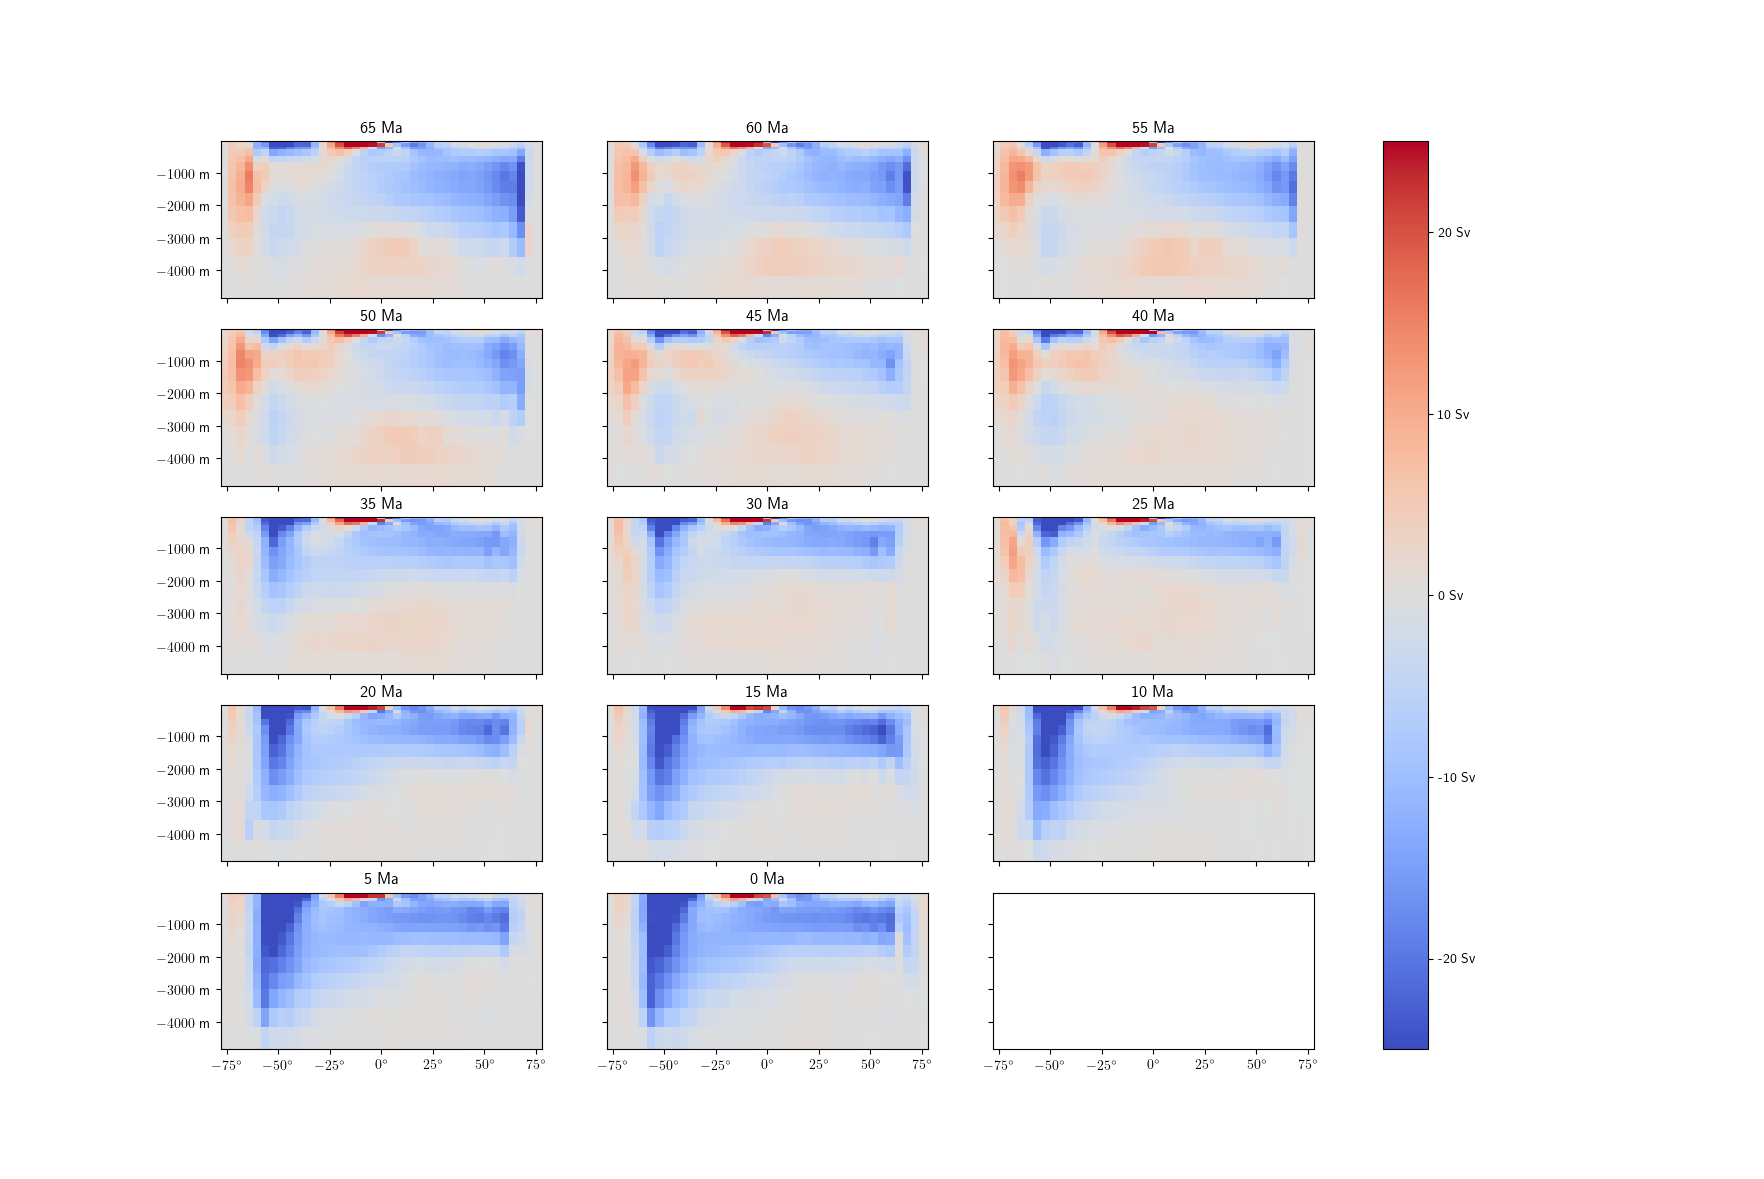
\includegraphics[width=\linewidth]{overturning_overview.png}
	\caption{test caption}
	\label{fig:example1}
\end{figure}
\end{multicols}
%example full width overturning
\begin{figure}[H]
	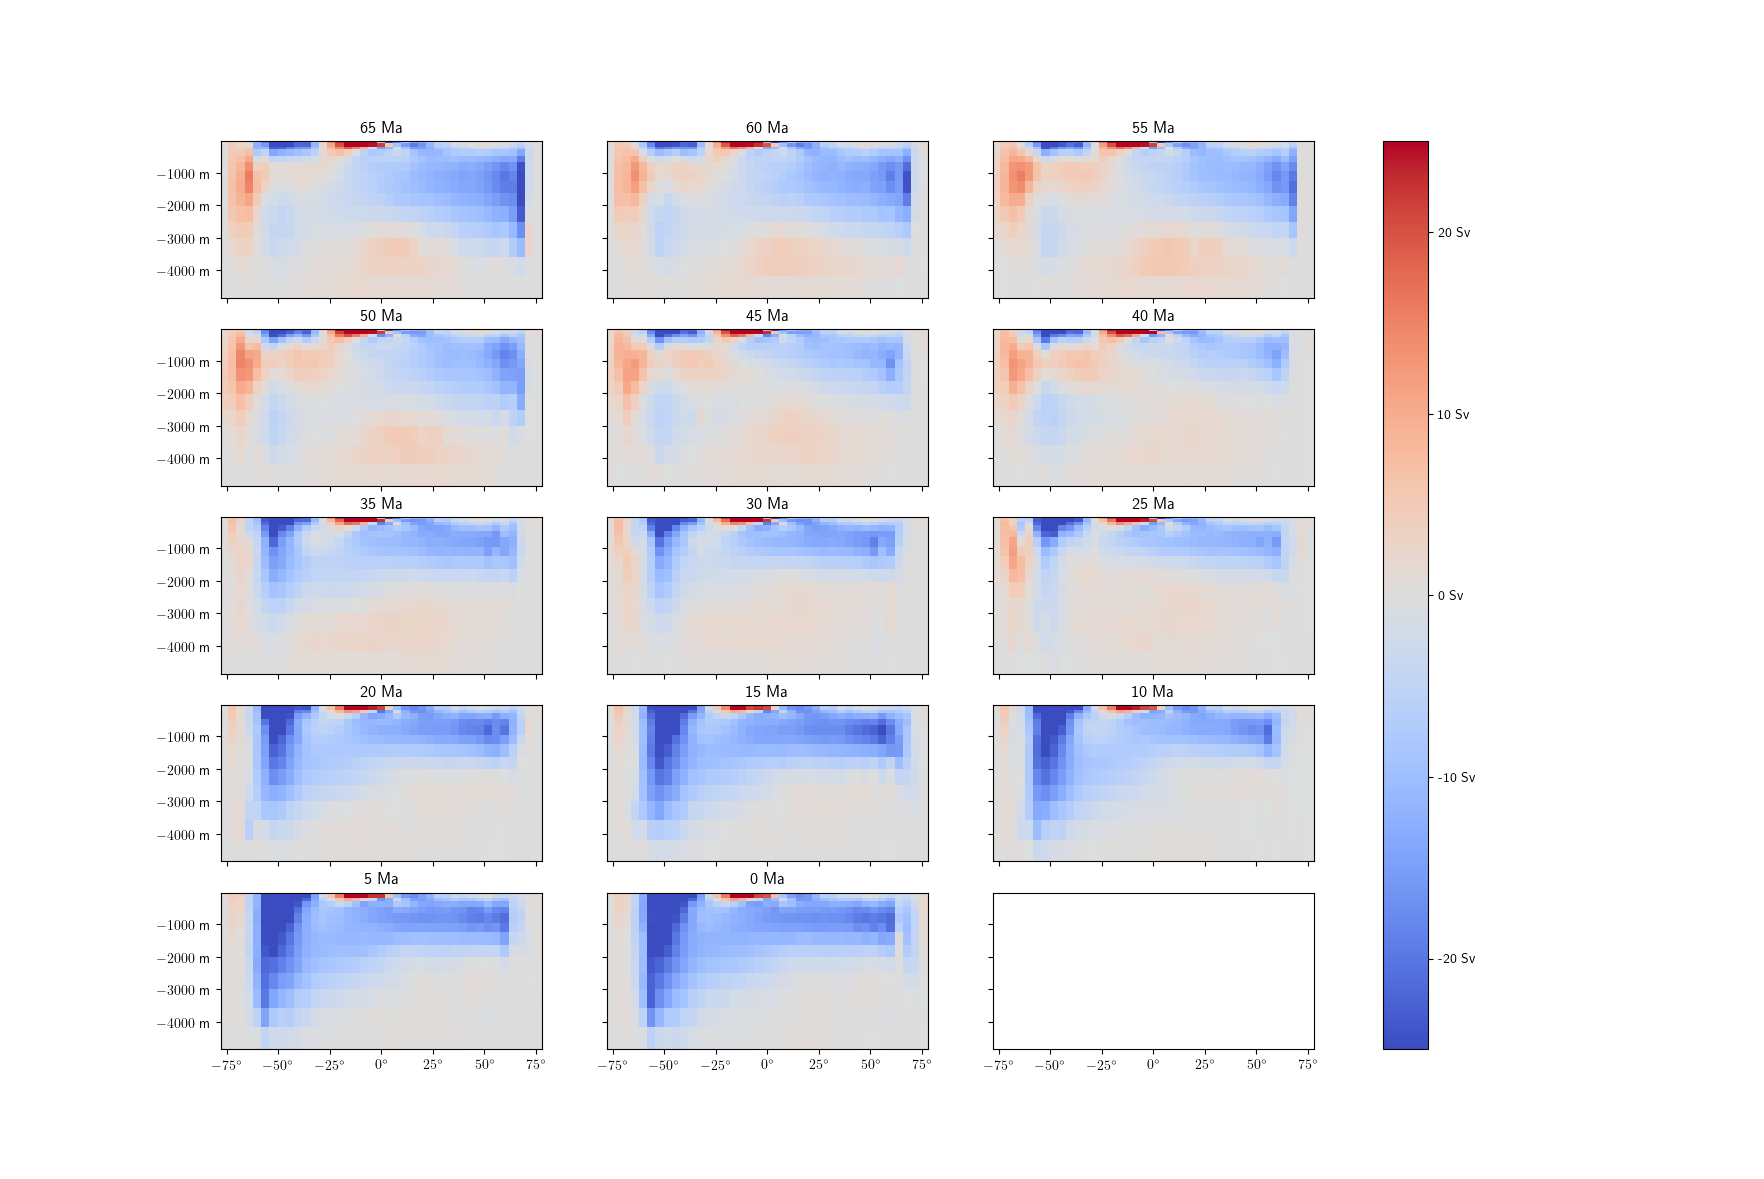
\includegraphics[width=\linewidth]{overturning_overview.png}
	\caption{test caption}
	\label{fig:example1}
\end{figure}

\begin{multicols}{2}

\printbibliography

\end{multicols}



\end{document}
